\documentclass{article}
\usepackage{graphicx}
\usepackage{amsmath,amsthm,amssymb}
\usepackage[font=small,labelfont=bf]{caption}
\usepackage{tikz}
\usetikzlibrary{calc, angles, quotes, shapes.geometric}
\usepackage{tkz-euclide}
\usepackage{float}
\usepackage[margin=1in]{geometry}
\usepackage{gensymb}
\usepackage{fancyhdr}
\pagestyle{fancy}
\fancyhead[R]{Enoch Yu}
\pagenumbering{gobble}
\usepackage{enumitem}
\newtheorem{theorem}{Theorem}[section]
\newtheorem{lemma}[theorem]{Lemma}
\newtheorem*{lemma*}{Lemma}
\newtheorem{sublemma}{Lemma}[section]
\newtheorem{proposition}{Proposition}
\newtheorem{corollary}{Corollary}[theorem]
\newenvironment{solution}{\begin{trivlist}\item[]{\bf Solution}}{\qed \end{trivlist}}
\newcommand{\verteq}{\rotatebox{90}{$\;\;=\;\;$}}
\newcommand*\circled[1]{\tikz[baseline=(char.base)]{
            \node[shape=circle,draw,inner sep=1pt] (char) {#1};}}
\newcommand{\triangled}[1]{\tikz[baseline=(char.base)]{
            \node[shape=regular polygon, regular polygon sides=3, draw, inner sep=0.2pt] (char) {#1};}}

\title{Problem Set 9}
\author{Enoch Yu}
\date{May 2025}

\begin{document}

\section*{2022 AMC 12A Problem 16}
A triangular number is a positive integer that can be expressed in the form $t_n=1+2+3+\cdots+n$, for some positive integer $n$. The three smallest triangular numbers that are also perfect squares are $t_1=1=1^2, t_8=36=6^2,$ and $t_{49}=1225=35^2$. What is the sum of the digits of the fourth smallest triangular number that is also a perfect square?
\\\\
$\textbf{(A)} ~6 \qquad\textbf{(B)} ~9 \qquad\textbf{(C)} ~12 \qquad\textbf{(D)} ~18 \qquad\textbf{(E)} ~27$
\begin{solution}
\\\\
\textbf{Key Word} Pell's Equation
\\\\
For arbitrary integers $k$, pairs of $(n,k)$ that satisfy $\frac{n(n+1)}{2}=k^2$ must be found. The equation could be rewritten as $n^2+n-2k^2=0$. Because $n$ and $k$ are positive integers, an impulse to find an cleaner relationship for trial and error is created. $(n+\frac{1}{2})^2-2k^2=\frac{1}{4}$. Multipying both sides by 4 may provide a better equation.
\[
(2n+1)^2-2(2k)^2=1
\]
Let $x=2n+1$ and $y=2k$ for cleaner view. $x^2-2y^2=1$ seems familiar. It is a specific Pell's Equation!!
\\\\
The fundamental solution is given by the problem which is $(2+1, 2\cdot1)$, or $(3,2)$. Because the general solution could be represented as $(x_i,y_i)=(x_1+y_1\sqrt{D})^i_{(i\ge1)}$, substitution is required.
\begin{align*}
(x_i,y_i)&=(3+2\sqrt{2})^i
\\\\
\text{For }i&=4, \\
(x_4,y_4)
&=(3+2\sqrt{2})^4 \\
&=(17+12\sqrt{2})^2 \\
&=577+408\sqrt{2}
\end{align*}
Therefore, $x_4=577$ and $y_4=408$. In another words, $n_4=288$ and $k_4=204$. Because $204^2=41616$, $4+1+6+1+6=\boxed{\textbf{(D)} ~18}$.
\end{solution}

\newpage
\section*{2022 AMC 12A Problem 20}
Isosceles trapezoid $ABCD$ has parallel sides $\overline{AD}$ and $\overline{BC},$ with $BC < AD$ and $AB = CD.$ There is a point $P$ in the plane such that $PA=1, PB=2, PC=3,$ and $PD=4.$ What is $\tfrac{BC}{AD}?$
\\\\
$\textbf{(A) }\frac{1}{4}\qquad\textbf{(B) }\frac{1}{3}\qquad\textbf{(C) }\frac{1}{2}\qquad\textbf{(D) }\frac{2}{3}\qquad\textbf{(E) }\frac{3}{4}$
\begin{solution}
\\\\
\textbf{Key Property} \\
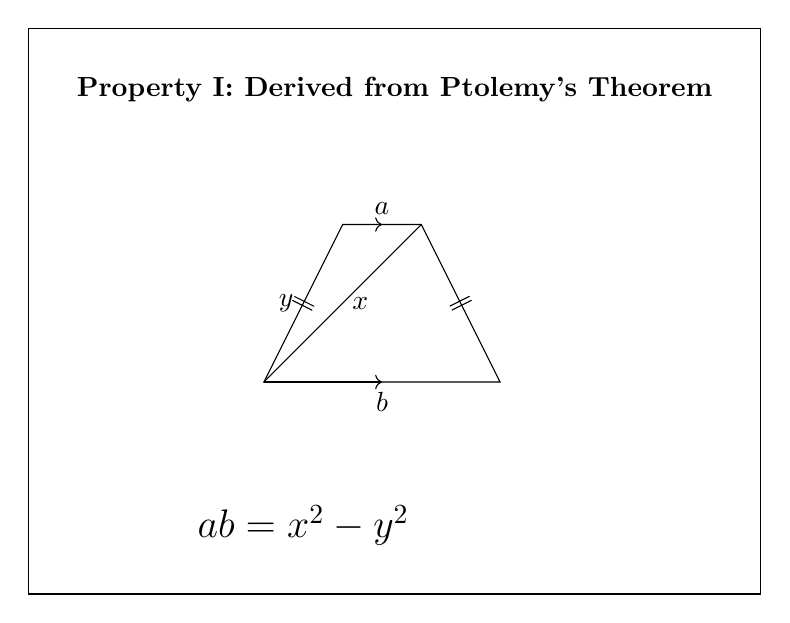
\begin{tikzpicture}
    \coordinate (A) at (0,0);
    \coordinate (B) at (1,2);
    \coordinate (C) at (2,2);
    \coordinate (D) at (3,0);
    
    \draw (A) -- (B) -- (C) -- (D) -- cycle;
    \draw (A) -- (C);
    
    \tkzMarkSegment[pos=.5, mark=||](A,B);
    \tkzMarkSegment[pos=.5, mark=||](C,D);

    \draw[->] (B) -- (1.5, 2);
    \draw[->] (A) -- (1.5,0);

    \node[above] at ($(B)!0.5!(C)$) {$a$};
    \node[below] at ($(A)!0.5!(D)$) {$b$};
    \node[right] at ($(A)!0.5!(C)$) {$x$};
    \node[left] at ($(A)!0.5!(B)$) {$y$};

    \node[anchor=north west] at (-2.5,4) {\textbf{Property I: Derived from Ptolemy's Theorem}};
    \node[anchor=south] at (0.5, -2.2) {\Large{$ab=x^2-y^2$}};

    \coordinate (SW) at (current bounding box.south west);
    \coordinate (NE) at (current bounding box.north east);
    \path[draw=black] 
    ($(SW)+(-0.5,-0.5)$) rectangle ($(NE)+(0.5,0.5)$);
\end{tikzpicture}
\\\\
General Rule of Thumb: \textcolor{red}{When an isosceles trapezoid is given, draw a symmetric pair!!}
\begin{center}
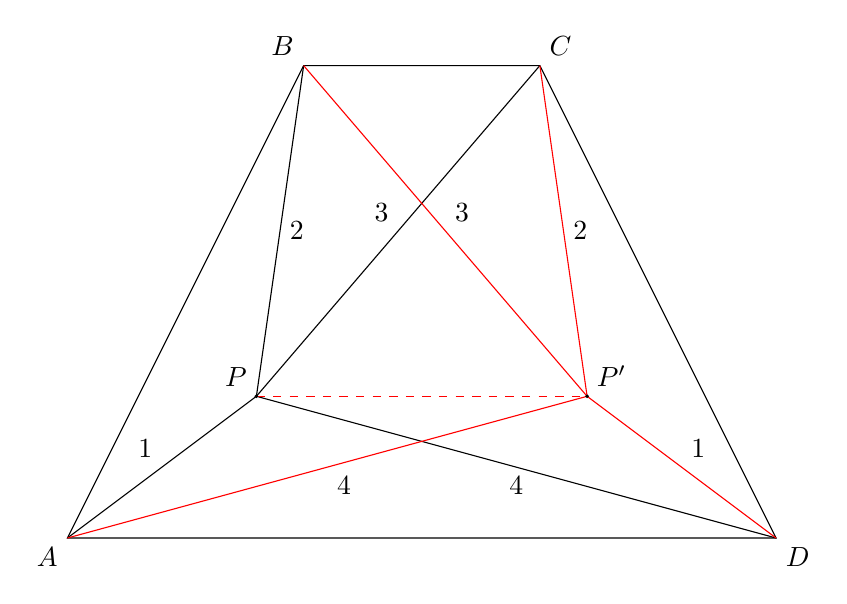
\begin{tikzpicture}[scale=3]

    \coordinate (A) at (0,0);
    \coordinate (B) at (1,2);
    \coordinate (C) at (2,2);
    \coordinate (D) at (3,0);
    \coordinate (P) at (0.8,0.6);
    \coordinate (P') at (2.2,0.6);
    
    \draw (A) -- (B) -- (C) -- (D) -- cycle;

    \draw (P) -- (A);
    \draw (P) -- (B);
    \draw (P) -- (C);
    \draw (P) -- (D);
    
    \draw[red] (P') -- (D);
    \draw[red] (P') -- (C);
    \draw[red] (P') -- (A);
    \draw[red] (P') -- (B);

    \draw[dashed, red] (P) -- (P');

    \node at (P)[circle,fill,inner sep=0.5pt]{};
    \node at (P')[circle,fill,inner sep=0.5pt]{};
    
    \node[below left] at (A) {$A$};
    \node[above left] at (B) {$B$};
    \node[above right] at (C) {$C$};
    \node[below right] at (D) {$D$};
    \node[above left] at (P) {$P$};
    \node[above right] at (P') {$P'$};

    \node[above left] at ($(P)!0.5!(A)$) {$1$};
    \node[right] at ($(P)!0.5!(B)$) {$2$};
    \node[above left] at ($(P)!0.5!(C)$) {$3$};
    \node[below] at ($(P)!0.5!(D)$) {$4$};

    \node[above right] at ($(P')!0.5!(D)$) {$1$};
    \node[right] at ($(P')!0.5!(C)$) {$2$};
    \node[above right] at ($(P')!0.5!(B)$) {$3$};
    \node[below right] at ($(P')!0.5!(A)$) {$4$};

\end{tikzpicture}
\end{center}
Using the property of isosceles trapezoid, it is evident that $BC \cdot PP'-=3^2-2^2=5$. Moreover, $PP' \cdot AD=4^2-1^1=15$. Therefore, $\frac{BC \cdot PP'}{PP' \cdot AD}=\frac{BC}{AD}=\frac{5}{15}=\boxed{\textbf{(B) }\frac{1}{3}}$.
\end{solution}

\end{document}
